% sage_latex_guidelines.tex V1.20, 14 January 2017

\documentclass[Afour,sagev,times]{sagej}
\usepackage{moreverb,url,adjustbox}
\usepackage[colorlinks,bookmarksopen,bookmarksnumbered,citecolor=red,urlcolor=red]{hyperref}
\usepackage{booktabs, multicol, makecell, amsmath,afterpage,multirow}

\usepackage{subcaption}
\usepackage{tikz,tabularx, adjustbox}
\usetikzlibrary{shapes.geometric, matrix,arrows,positioning,calc,intersections}

\newcommand\BibTeX{{\rmfamily B\kern-.05em \textsc{i\kern-.025em b}\kern-.08em
T\kern-.1667em\lower.7ex\hbox{E}\kern-.125emX}}
\def\volumeyear{2016}

\newcommand{\ROOT}{./}

\begin{document}

\runninghead{Optimal design of laminate by genetic algorithm}

\title{A technique for constrained optimization of cross ply laminates using a new variant of genetic algorithm}

\author{Huiyao Zhang\affilnum{1} and Atsushi Yokoyama\affilnum{2}}

\affiliation{\affilnum{1}Department of Fiber Science and Engineering, Kyoto
	Institute of Technology\\
\affilnum{2}Department of Fiber Science and Engineering, Kyoto Institute of
Technology}

\corrauth{Atsushi Yokoyama, Department of Fiber Science and Engineering, Kyoto Institute of Technology,
 Matsugasaki, Sakyo-ku, Kyoto, 606-8585,JAPAN
}

\email{yokoyama@kit.ac.jp}

\begin{abstract}
	The main challenge presented by the laminate composite design is the laminate
layup, involving a set of fiber orientations, composite material systems, and
stacking sequences. In nature, it is a combinatorial optimization problem that
can be solved by the genetic algorithm (GA). In this present study, a new
variant of the GA is proposed for the optimal design by modifying the selection
strategy.  To check the feasibility of a laminate subject to in-plane loading,
the effect of the fiber orientation angles and material components on the first
ply failure is studied. Then we compare the experiment results with works in
other literature.

\end{abstract}

\keywords{Laminate composite, Classical lamination theory, Genetic algorithm, Optimal design}

\maketitle


\section{Introduction}
Composite materials offer improved strength, stiffness, fatigue, corrosion resistance, etc. over
conventional materials, and are widely used as materials for applications ranging from the automotive to shipbuilding
industry, electronic packaging to golf clubs, and medical equipment to homebuilding. However, the high
cost of fabrication of composites is a critical drawback to its application. For example, the
graphite/epoxy composite part may cost as much as $650$ to $900$ per kilogram. In contrast, the price
of glass/epoxy is about 2.5 times less. Manufacturing techniques such as sheet molding compounds and
structural reinforcement injection molding is used to lower the  costs for manufacturing automobile parts.
An alternative approach is using hybrid composite materials.


The mechanical performance of a laminate composite is affected by a wide range of factors such as the
thickness, material, and orientation of each lamina. Because of manufacturing limitations, all these
variables are usually limited to a small set of discrete values. For example, the ply thickness is fixed
and ply orientation angles are limited to a set of angles such as 0, 45, and 90 degrees in practice. So
the search process for the optimal design is a discrete optimization problem that can be solved by the
GA. To tailor a laminate composite, the GA has been successfully applied to solve laminate design
problems\cite{riche1993optimization,nagendra1996improved,sadagopan1998application,todoroki1998stacking,liu2000permutation,sivakumar1998optimum,walker2003technique,lin2004stacking,kang2005minimum,murugan2007target,akbulut2008optimum}.
The GA simulates the process of natural evolution, including selection, crossover, and mutation
according to Darwin's principal of ''survival of the fittest''. The known advantages of GAs are the
following: (i): GAs are not easily trapped in local optima and can obtain the global
optimum. (ii): GAs do not need gradient information and can be applied to discrete optimization
problems. (iii): GAs can not only find the optimal value in the domain but also maintain a
set of optimal solutions. However, the GA also has some disadvantages, for example, the GA
needs to evaluate the target functions many times to achieve the optimization, and the cost of the
search process is high. The GA consists of some basic parts, the coding of the design variable,
the selection strategy, the crossover operator, the mutation operator, and how to deal with constraints. For the
variable design part, there are two methods to deal with the representation of design variables, namely,
binary string and real value representation\cite{riche1993optimization,todoroki1998stacking}.
Michalewicz\cite{zbigniew1996genetic} claimed that the performance of floating-point representation was
better than binary representation in the numerical optimization problem. Selection strategy plays a
critical role in the GA, which determines the convergence speed and the diversity of the population. To
improve search ability and reduce search costs, various selection methods have been invented, and they
can be divided into four classes: proportionate reproduction, ranking, tournament, and
genitor(or ''steady state'') selection. In the optimization of laminate composite design, the roulette
wheel\cite{riche1993optimization,seresta2007optimal}, where the possibility of an individual to be
chosen for the next generation is proportional to the fitness.
Soremekun et al.\cite{soremekun2001composite} showed that the generalized elitist strategy outperformed a
single individual elitism in some special cases.

Data structure, repair strategies and penalty functions\cite{le1995improved} are the most commonly used
approaches to resolve constrained problems in the optimization of composite structures. Symmetric
laminates are widely used in practical scenarios, and data structures can be used to fulfill symmetry
constraints, which consists of coding half of the laminate and considering the rest with the
opposite orientation. Todoroki\cite{todoroki1998stacking} introduced a repair strategy that can scan the chromosome and
repair the gene on the chromosome if it does not satisfy the contiguity constraint. The comparison of
repair strategies in a permutation GA with the same orientation was presented by Liu et al.\cite{liu2000permutation}, and it
showed that the Baldwinian repair strategy can substantially reduce the cost of constrained optimization.
Haftka and Todoroki\cite{riche1993optimization} used the GA to solve the laminate stacking sequence problem using a penalty function subject to
buckling and strength constraints.

In typical engineering applications, composite materials are under very complicated loading
conditions, not only inplane loading but also out-of-plane loading. Most of the studies on the
optimization of the laminate composite material minimized the
thickness\cite{abu1998optimum,walker2003technique},
weight\cite{fang1993design,deka2005multiobjective,park2008improved}, and cost and
weight\cite{deka2005multiobjective,omkar2008artificial}, or maximized the static strength of
the composite laminates for a targeted
thickness\cite{walker2003technique,lin2004stacking,kim2007development,gholami2020multi}. 
In the present study,
the cost and weight of laminates are minimized by modifying the objective function.

To check the feasibility of a laminate composite by imposing a strength constraint, failure
analysis of a laminate is performed by applying suitable failure criteria. The failure criteria of
laminated composites can be classified into three classes: non-interactive theories (e.g., maximum
strain), interactive theories (e.g., Tsai-wu), and partially interactive theories (e.g., Puck failure
criterion). Previous researchers adopted the first-ply-failure approach using Tsai-wu
failure
theory\cite{massard1984computer,reddy1987first,fang1993design,soeiro1994multilevel,pelletier2006multi,jadhav2007parametric,omkar2008artificial,choudhury2019failure},
Tsai-Hill\cite{martin1987optimum,soares1995discrete}, the maximum stress\cite{watkins1987multicriteria}, or the maximum strain\cite{watkins1987multicriteria}
static failure criteria. Akbulut\cite{akbulut2008optimum} used the GA to minimize the thickness of composite laminates with
Tsai-Hill and maximum stress failure criteria, and the advantage of this method is it avoid spurious
optima. Naik et al.\cite{naik2008design}
minimized the weight of laminated composites under restrictions with a
failure mechanism-based criterion based on the maximum strain and Tsai-wu. In the present study, Tsai-wu
Static failure criteria are used to investigate the feasibility of a laminate composite.

\section{Stress and Strain in a Laminate}
\begin{figure*}[!htb]
	\centering
	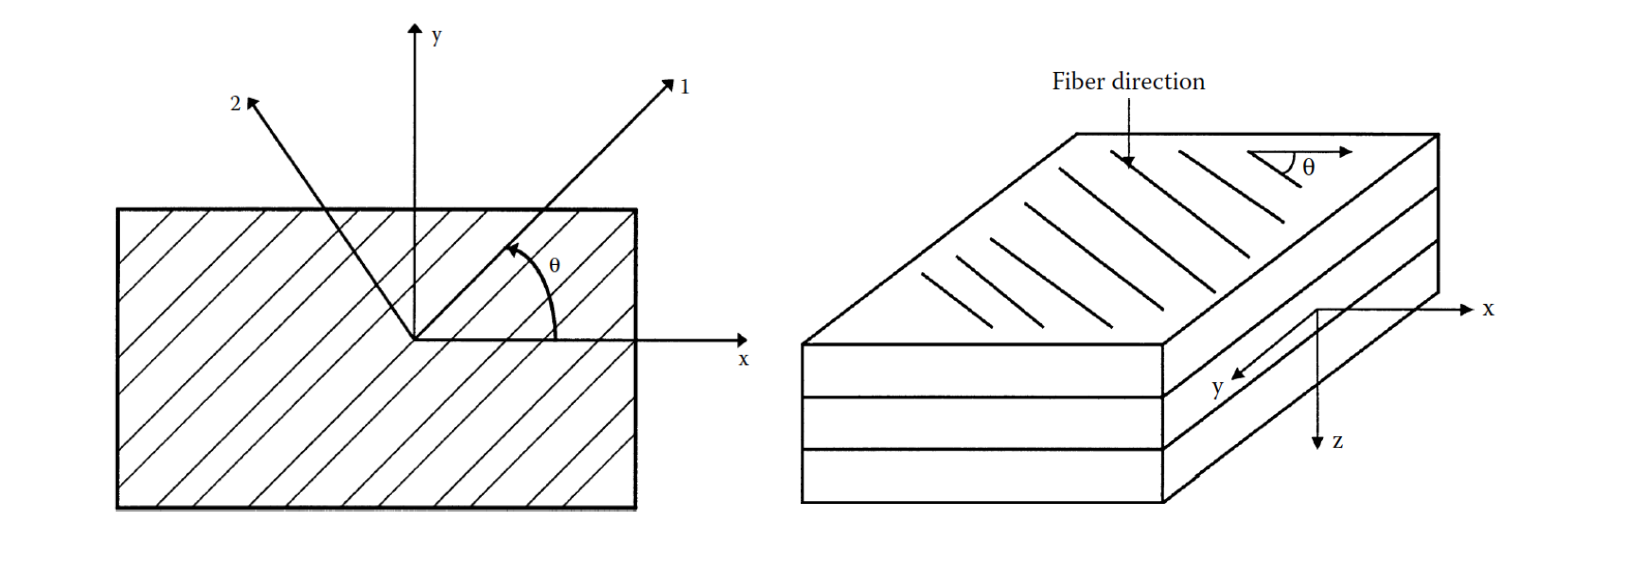
\includegraphics[width=\linewidth]{\ROOT/fig/lamina_local_global_axes.png}
\caption{Lamina}
  	\label{fig:lamina}
\end{figure*}

\begin{figure} \centering
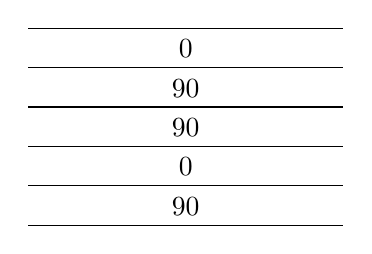
\begin{tikzpicture}
	\draw (0,0) -- (4,0);
	\draw (0,-0.5) -- (4,-0.5) node[midway, above] {$0$};
	\draw (0,-1) -- (4,-1) node[midway, above] {$90$} ;
	\draw (0,-1.5) -- (4,-1.5) node[midway, above] {$90$};
	\draw (0,-2) -- (4,-2) node[midway, above] {$0$};
	\draw (0,-2.5) -- (4,-2.5) node[midway, above] {$90$};
\end{tikzpicture}
\caption{Model for cross ply laminate.}
\end{figure}

A laminate structure consists of multiple lamina bonded together through their thickness.
Considering a laminate composite plate that is symmetric to its middle plane subject to in-plane
loading of extension, shear, bending and torsion, the classical lamination theory (CLT) is taken to
calculate the stress and strain in the local and global axes of each ply, as shown in
Fig.~\ref{fig:lamina}.




\subsection{Stress and Strain in a Lamina}
For a single lamina, the stress-strain relation in local axis 1-2 is:
\begin{equation}
    \begin{bmatrix}
        \sigma _1\\
        \sigma _2\\
        \tau_{12}
    \end{bmatrix}
    =
    \begin{bmatrix}
        Q_{11} & Q_{12} & 0\\
        Q_{12} & Q_{22} & 0\\
        0      &  0     & Q_{66}
    \end{bmatrix}
    \begin{bmatrix}
        \varepsilon_1\\
        \varepsilon_2\\\gamma_{12}
    \end{bmatrix}
\end{equation}
where $Q_{ij} $are the stiffnesses of the lamina that are related

to engineering elastic constants given by
\begin{equation}
    \begin{split}
    &Q_{11}=\frac{E_1}{1-v_{12}v_{21}}\\
    &Q_{22}=\frac{E_2}{1-v_{12}v_{21}}\\
    &Q_{66}=G_{12}\\
    &Q_{12}=\frac{v_{21}E_2}{1-v_{12}v_{21}}\\
    \end{split}
\end{equation}

where $E_1, E_2, v_{12}, G_{12} $ are four independent engineering elastic constants, which are defined as follows: $E_1 $ is the longitudinal Young's modulus, $E_2 $ is the transverse Young's modulus, $v_{12} $ is the major Poisson's ratio, and $G_{12} $ is the in-plane shear modulus.

Stress strain relation in the global x-y axis:
\begin{equation}\left[\begin{array}{l}\sigma _{x} \\ \sigma _{y} \\ \tau_{xy}\end{array}\right]=\left[\begin{array}{lll}\bar{Q}_{11} & \bar{Q}_{12} & \bar{Q}_{16}\\ \bar{Q}_{12} & \bar{Q}_{22} & \bar{Q}_{26} \\ \bar{Q}_{16} & \bar{Q}_{26} &\bar{Q}_{66}\end{array}\right]\left[\begin{array}{l}\varepsilon_{x} \\ \varepsilon_{y}\\ \gamma_{x y}\end{array}\right]
\end{equation}
where

\begin{equation}
	\begin{array}{l}
		\resizebox{.35\textwidth}{!}{$\bar{Q}_{11}=Q_{11} c^{4}+Q_{22} s^{4}+2\left(Q_{12}+2
		Q_{66}\right) s^{2} c^{2}$} \\

		\resizebox{.35\textwidth}{!}{$\bar{Q}_{12}=\left(Q_{11}+Q_{22}-4 Q_{66}\right) s^{2}
		c^{2}+Q_{12}\left(c^{4}+s^{2}\right)$} \\

		\resizebox{.35\textwidth}{!}{$\bar{Q}_{22}=Q_{11} s^{4}+Q_{22} c^{4}+2\left(Q_{12}+2
		Q_{66}\right) s^{2} c^{2}$} \\

		\resizebox{.4\textwidth}{!}{$\bar{Q}_{16}=\left(Q_{11}-Q_{12}-2 Q_{66}\right) c^{3} s-\left(Q_{22}-Q_{12}-2Q_{66}\right) s^{3} c$}
		 \\ 
		\resizebox{.4\textwidth}{!}{$\bar{Q}_{26}=\left(Q_{11}-Q_{12}-2 Q_{66}\right) c s^{3}-\left(Q_{22}-Q_{12}-2 Q_{66}\right)c^{3} s$}
		 \\ 
	\resizebox{.4\textwidth}{!}	{$\bar{Q}_{66}=\left(Q_{11}+Q_{22}-2 Q_{12}-2 Q_{66}\right)
	s^{2}c^{2}+Q_{66}\left(s^{4}+c^{4}\right)$}\\
	\end{array}
\end{equation}


The c and s denotes $cos\theta $ and $sin\theta $.

The local and global stresses in an angle lamina are related

to each other through the angle of the lamina $\theta $
\begin{equation}\left[\begin{array}{l}\sigma _{1} \\ \sigma _{2} \\ \tau_{12}\end{array}\right]=[T]\left[\begin{array}{l}\sigma _{x} \\ \sigma _{y} \\\tau_{xy}\end{array}\right]
\end{equation}

where
\begin{equation}[T]=\left[\begin{array}{ccc}c^{2} & s^{2} & 2 s c \\ s^{2} & c^{2} & -2 s c \\ -s c & s c &c^{2}-s^{2}\end{array}\right] 
\end{equation}



\subsection{Stress and Strain in a Laminate}
\begin{equation} \label{eq:force_and_moments}
	\begin{array}{l}
		\begin{aligned}
	\begin{bmatrix}
		N_x \\
		N_y \\
		N_{xy}
	\end{bmatrix}
	&=
	\begin{bmatrix}
		A_{11} & A_{12} & A_{16} \\
		A_{12} & A_{22} & A_{26} \\
		A_{16} & A_{26} & A_{66} 
	\end{bmatrix}
    \begin{bmatrix}
		\varepsilon_x^0 \\
        \varepsilon_y^0 \\
		\gamma_{xy}^0
    \end{bmatrix}   \\
	&+               
	\begin{bmatrix}
		B_{11} & B_{12} & B_{16} \\
		B_{11} & B_{12} & B_{16} \\
		B_{16} & B_{26} & B_{66} 
	\end{bmatrix}
	\begin{bmatrix}
		k_x \\
		k_y \\
		k_{xy} 
	\end{bmatrix}  \\
\end{aligned} \\ \\
\begin{aligned}
	\begin{bmatrix}
		M_x \\
		M_y \\
		M_{xy}
	\end{bmatrix}
	&=
	\begin{bmatrix}
		B_{11} & B_{12} & B_{16} \\
		B_{12} & B_{22} & B_{26} \\
		B_{16} & B_{26} & B_{66} 
	\end{bmatrix}
    \begin{bmatrix}
		\varepsilon_x^0 \\
        \varepsilon_y^0 \\
		\gamma_{xy}^0
    \end{bmatrix} \\ 
	&+  
	\begin{bmatrix}
		D_{11} & D_{12} & D_{16} \\
		D_{11} & D_{12} & D_{16} \\
		D_{16} & D_{26} & D_{66} 
	\end{bmatrix}
	\begin{bmatrix}
		k_x \\
		k_y \\
		k_{xy} 
	\end{bmatrix}
\end{aligned}
	\end{array}
\end{equation}


$N_x,N_y $  - normal force per unit length

$N_{xy} $  - shear force per unit length

$M_x, M_y $ - bending moment per unit length

$M_{xy} $  - twisting moments per unit length

$\varepsilon^{0}, k $- mid plane strains and curvature of a laminate in x-y coordinates

The mid plane strain and curvature is given by
\begin{equation}
    \begin{split}
    &A_{ij}=\sum_{k=1}^{n}(\overline{Q_{ij}})_k(h_k-h_{k-1})  i=1,2,6, j=1,2,6\\
    &B_{ij}=\frac{1}{2}\sum_{k=1}^{n}(\overline{Q_{ij}})_k(h^2_k - h_{k-1}^2)  i=1,2,6, j=1,2,6\\
    &D_{ij}=\frac{1}{3}\sum_{k=1}^{n}(\overline{Q_{ij}})_k(h^3_k - h_{k-1}^3) i=1,2,6, j=1,2,6\\
    \end{split}
\end{equation}

The [A], [B], and [D] matrices are called the extensional, coupling, and bending stiffness matrices.

\section{Failure Theory}

\subsection{Failure Process}
A laminate will fail under increasing mechanical loading; however, the procedure of laminate failure may not
be catastrophic.
 In some cases, some layers fail first, and the rest are able to continue to take additional loading
 until all the plies fail. A ply is fully discounted when a ply fails; then, the ply is replaced
by a near zero stiffness and strength. 
The procedure for finding the first ply failure in the present
study follows the fully discounted method:

\begin{enumerate}
\item Compute the reduced stiffness matrix [Q] referred to as the local axis for each ply using its four engineering elastic constants $E_1 $, $E_2 $, $E_{12} $, and $G_{12} $.

\item Calculate the transformed reduced stiffness $[\bar{Q}] $ referring to the global coordinate system (x, y) using the reduced stiffness matrix [Q] obtained in step 1 and the ply angle for each layer.

\item  Given the thickness and location of each layer, the three laminate stiffness matrices [A], [B], and [D] are determined.

\item  Apply the forces and moments, $[N]_{xy}, [M]_{xy} $ solve
Equation \ref{eq:force_and_moments}, and calculate the middle plane strain $[\sigma ^{0}]_{xy} $ and curvature $[k]_{xy} $.

\item Determine the local strain and stress of each layer under the applied load.

\item  Use the ply-by-ply stress-strain and related failure theories to determine the strength ratio.
\end{enumerate}

\subsection{Tsai-wu Failure Theory}

Many different theories about the failure of an angle lamina have been developed for a
unidirectional lamina, such as the maximum stress failure theory, maximum strain failure theory,
Tsai-Hill failure theory, and Tsai-Wu failure theory. The failure theories of a lamina are based on
the stresses in the local axes in the material. There are four normal strength parameters and one shear
stress for a unidirectional lamina. The five strength parameters are:

$(\sigma _1^{T})_{ult}= $ ultimate longitudinal tensile strength

$(\sigma _1^{C})_{ult}= $ ultimate longitudinal compressive strength

$(\sigma _2^{T})_{ult}= $ ultimate transverse tensile strength

$(\sigma _2^{C})_{ult}= $ ultimate transverse compressive strength 

$(\tau_{12})_{ult}= $ and ultimate in-plane shear strength

In the present study, Tsai-wu failure theory is taken to decide whether a lamina fails,
because this theory is more general than the Tsai-Hill failure theory, which considers two
different situations, the compression and tensile strengths of a lamina. A lamina is considered to fail
if \begin{equation} \label{eq:tsai_wu}
\begin{split}
	H_1 \sigma_1  & + H_2 \sigma_2 + H_6 \tau_{12} + H_{11}\sigma_1^2 + H_{22} \sigma_2^2 \\
				  & + H_{66}  \tau_{12}^2 + 2H_{12}\sigma_1\sigma_2 < 1
\end{split}
\end{equation}

is violated, where

\begin{equation} \label{eq:sr}S R=\frac{\text {Maximum Load Which Can Be Applied}}{\text {Load Applied}}
\end{equation}


\section{Genetic algorithm model}

\input{Figures/chapter4/part1/fig/chapter3_ngam.tex}
\input{Figures/chapter4/part1/fig/chapter3_ogam.tex}
The genetic algorithm starts with multiple individuals with limited chromosome lengths, in
which maybe none of these individuals fulfill the constraints. The GA is
assumed to derive appropriate offspring based on the initial population as the
GA continues. The traditional way to handle the constrained search of the GA is
either to introduce repair strategies or to use a penalty function. Fig.
\ref{fig:old_ga_model} shows the classic flow chart of a GA framework, which
includes selection, crossover, and mutation operators. However, GA is originally
proposed to solve unconstrained problems; therefore, we suggest a new approach 
to address the constrained GA search problem in an unconstrained way. 

Because of the existence of constraints, the population not only can be sorted
by the fitness (obtained by the objective function) but also sorted by
the constraint value obtained by the constraint function (assuming a constraint
function exists), so the parents of the next generation can be chosen by the
following three approaches. First, the population is sorted by fitness in
ascending order, and individuals with smaller fitness are selected. These
selected individuals form a group named as a proper group. Second, remove
individual which satisfies constraints, and sort population by the difference
between the individual's constraint value and the threshold of the constraint
in descending order, and individuals with bigger differences are chosen to be
the parents of the next generation. The group which forms are called potential
group, and an individual from this group is referred to as a potential
individual.  Third, the population is sorted by fitness from low to high after
removing individuals which fails to fit the constraints, select individuals
with bigger fitness, and these individuals form the proper group.  So the final
parents' pool is consists of three groups, active group, potential group, and
proper group.  The number of active individuals, potential individuals, and
proper individuals are called, respectively, active number, potential numbers,
and proper number. 

Each group in the parents' population has its role in the searching
process. The problem within traditional GA is premature and has weak local
search ability, therefore, traditional GAs are more likely to get stuck in a
local optimum. To prevent the GA from experiencing early convergence and to
improve the local search performance, the active group is proposed to overcome
this problem. As its name suggests, this group would always live in the
population.  Because both active individual's fitness and constraint value are small,
each individual can be treated as an independent gene clip. So their existence
enriches the gene clip variety of the mating pool. The offspring of two active
individuals are more likely to be an active individual, which can maintain the
active group.

For an individual in the potential group, it doesn't satisfy the constraint,
however, it's supposed to evolve into a proper individual after multiple
generations by modifying its chromosome structure or length. The crossover
operation could happen between a potential individual with an active
individual, or a potential individual, or a proper individual. The child of an
active individual and a potential individual is more likely to be a potential individual,
and this active individual could inject a new gene clip into this potential
individual, therefore providing a new evolution direction. 


A proper individual means a feasible solution, which fulfills all the constraints. 
However, there are still some drawbacks within it, for example, its fitness is low.
The crossover operation could happen between a proper individual and any other individuals.


The mutation operator for an active group is different from the potential group
and proper group because their roles in the searching process are different:
the target of the potential group and proper group is to obtain a feasible
solution; however, the role of the active group is to maintain the variety of gene
clips in the mating pool. 

Fig.\ref{fig:model} shows the flow chart of the proposed GA. First, the
population is divided into three groups, active group, potential group, and
proper group by the above-mentioned method. Second, select an appropriate number of
individuals from each group as parents, and the various selection scheme can be
taken for each group. 


The searching process can be divided into two phases according to whether
proper individuals are generated or not. During the initial stage, no individual in
the population is appropriate, which means the number of individuals in the
proper group is zero. Both active group and potential group are full. After a
couple of generations, some proper individuals could be produced. Then, the GA
comes to its second phase, the number of proper individuals begins to increase,
finally, the number in the proper group reaches its upper bound. 


\section{Experiment}
First, we formulate a constrained problem by searching the optimal stacking
sequence of cross ply laminate under in-plane loading whose strength ratio is
not less than 2.  Each lamina dimensions $1000 \times 1000 \times 0.165 mm^3$
is adopted in this experiment, each graphite/epoxy,  and glass/epoxy layer is
assumed to cost 2.5 and 1 monetary units, respectively. The other material
properties are shown in Table \ref{tab:mat}. 


\subsection{Problem formulation}

In the present experiment, the optimal composite sequences, and the number of
layers for a targeted strength ratio under in-plane loading conditions are
investigated.  The aim is to minimize the mass of a laminate composite for a
targeted strength ratio based on the Tsai-wu failure theory. The design
variables are the ply angles and the number of layers.  Ply orientation
restricted to a discrete set of angles ($0, \text{ and } 90 \text{ degrees} $).
The problem can be formulated as the following equation

Find: $\{\theta_k, n\}$ $\theta_k \in \{ 0,90\}$

Minimize: weight

Subject to: strength ratio


\subsection{GA Operation}

\begin{figure}[!htb]
\setlength{\fboxsep}{0pt}%
\setlength{\fboxrule}{0pt}%
\begin{center}
\resizebox{.95\linewidth}{!}{
		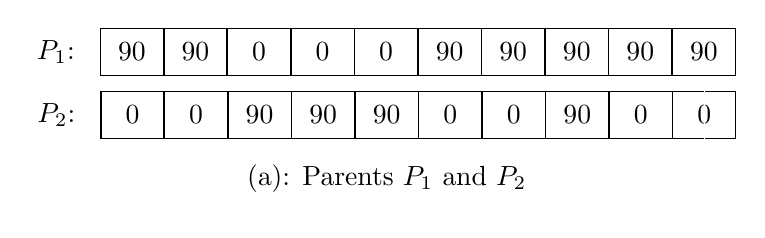
\begin{tikzpicture}
		\tikzstyle{rec} = [rectangle, minimum width=0.8cm,minimum height=0.6cm, text
		centered, draw=black]
			\node (gene11) [rec] {90};
			\node (gene2) [rec] at ($(gene11.east)+(0.4cm,0)$)  {90};
			\node (gene3) [rec] at ($(gene2.east)+(0.4cm,0)$)  {0};
			\node (gene4) [rec] at ($(gene3.east)+(0.4cm,0)$)  {0};
			\node (gene5) [rec] at ($(gene4.east)+(0.4cm,0)$)  {0};
			\node (gene6) [rec] at ($(gene5.east)+(0.4cm,0)$)  {90};
			\node (gene7) [rec] at ($(gene6.east)+(0.4cm,0)$)  {90};
			\node (gene8) [rec] at ($(gene7.east)+(0.4cm,0)$)  {90};
			\node (gene9) [rec] at ($(gene8.east)+(0.4cm,0)$)  {90};
			\node (last) [rec] at ($(gene9.east)+(0.4cm,0)$)  {90};
			\node[text width=1cm] at ($(gene11.west)+(-0.3cm,0)$) {$P_1$:};
			\node (gene1) [rec] at ($(gene11.east)+(-0.4cm,-0.8cm)$) {0};
			\node (gene2) [rec] at ($(gene1.east)+(0.4cm,0)$)  {0};
			\node (gene3) [rec] at ($(gene2.east)+(0.4cm,0)$)  {90};
			\node (gene4) [rec] at ($(gene3.east)+(0.4cm,0)$)  {90};
			\node (gene5) [rec] at ($(gene4.east)+(0.4cm,0)$)  {90};
			\node (gene6) [rec] at ($(gene5.east)+(0.4cm,0)$)  {0};
			\node (gene7) [rec] at ($(gene6.east)+(0.4cm,0)$)  {0};
			\node (gene8) [rec] at ($(gene7.east)+(0.4cm,0)$)  {90};
			\node (gene9) [rec] at ($(gene8.east)+(0.4cm,0)$)  {0};
			\node (gene10) [rec] at ($(gene9.east)+(0.4cm,0)$)  {0};
			\node[text width=1cm] at ($(gene1.west)+(-0.3cm,0)$) {$P_2$:};
			\draw[-,white] ($(gene10.north)$)-- ++(0,-1.5cm);
			\node (label1) at ($(gene5.south)+(0cm,-0.5cm)$) {(a): Parents $P_1$ and $P_2$};
		\end{tikzpicture}
}

% offspring
\resizebox{.95\linewidth}{!}{
		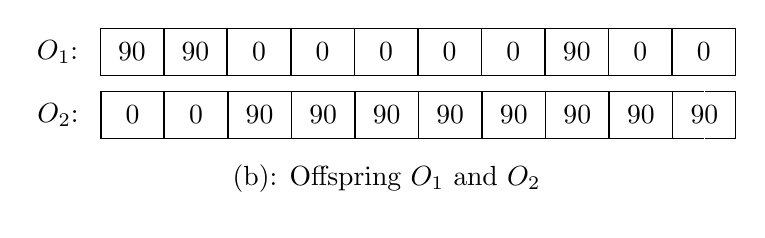
\begin{tikzpicture}
			\tikzstyle{rec} = [rectangle, minimum width=0.8cm,minimum height=0.6cm, text
			centered, draw=black]
			\node (gene11) [rec] {90};
			\node (gene2) [rec] at ($(gene11.east)+(0.4cm,0)$) {90};
			\node (gene3) [rec] at ($(gene2.east)+(0.4cm,0)$)  {0};
			\node (gene4) [rec] at ($(gene3.east)+(0.4cm,0)$)  {0};
			\node (gene5) [rec] at ($(gene4.east)+(0.4cm,0)$)  {0};
			\node (gene6) [rec] at ($(gene5.east)+(0.4cm,0)$)  {0};
			\node (gene7) [rec] at ($(gene6.east)+(0.4cm,0)$)  {0};
			\node (gene8) [rec] at ($(gene7.east)+(0.4cm,0)$)  {90};
			\node (gene9) [rec] at ($(gene8.east)+(0.4cm,0)$)  {0};
			\node (last) [rec] at ($(gene9.east)+(0.4cm,0)$)  {0};
			\node[text width=1cm] at ($(gene11.west)+(-0.3cm,0)$) {$O_1$:};
			\node (gene1) [rec] at ($(gene11.east)+(-0.4cm,-0.8cm)$) {0};
			\node (gene2) [rec] at ($(gene1.east)+(0.4cm,0)$)  {0};
			\node (gene3) [rec] at ($(gene2.east)+(0.4cm,0)$)  {90};
			\node (gene4) [rec] at ($(gene3.east)+(0.4cm,0)$)  {90};
			\node (gene5) [rec] at ($(gene4.east)+(0.4cm,0)$)  {90};
			\node (gene6) [rec] at ($(gene5.east)+(0.4cm,0)$)  {90};
			\node (gene7) [rec] at ($(gene6.east)+(0.4cm,0)$)  {90};
			\node (gene8) [rec] at ($(gene7.east)+(0.4cm,0)$)  {90};
			\node (gene9) [rec] at ($(gene8.east)+(0.4cm,0)$)  {90};
			\node (gene10) [rec] at ($(gene9.east)+(0.4cm,0)$)  {90};
			\node[text width=1cm] at ($(gene1.west)+(-0.3cm,0)$) {$O_2$:};
			\draw[-,white] ($(gene10.north)$)-- ++(0,-1.5cm);
			\node (label1) at ($(gene5.south)+(0cm,-0.5cm)$) {(b): Offspring $O_1$ and $O_2$};
		\end{tikzpicture}
}

%mutation
\resizebox{.95\linewidth}{!}{
	\begin{tikzpicture}
	\tikzstyle{rec} = [rectangle, minimum width=0.8cm,minimum height=0.6cm, text
	centered, draw=black]
		\tikzstyle{rec} = [rectangle, minimum width=0.8cm,minimum height=0.6cm, text
		centered, draw=black]
		%\draw[help lines](-3,-3) grid (4,4);
		\node (gene11) [rec] {90};
		\node (gene2) [rec] at ($(gene11.east)+(0.4cm,0)$)  {90};
		\node (gene3) [rec] at ($(gene2.east)+(0.4cm,0)$)  {90};
		\node (gene4) [rec] at ($(gene3.east)+(0.4cm,0)$)  {$\cdots$};
		\node (gene5) [rec] at ($(gene4.east)+(0.4cm,0)$)  {90};
		\node (gene6) [rec] at ($(gene5.east)+(0.4cm,0)$)  {90};
		\node (gene7) [rec] at ($(gene6.east)+(0.4cm,0)$)  {0};
		\node (gene8) [rec] at ($(gene7.east)+(0.4cm,0)$)  {$\cdots$};
		\node (gene9) [rec] at ($(gene8.east)+(0.4cm,0)$)  {0};
		\node (last) [rec] at ($(gene9.east)+(0.4cm,0)$)  {0};
		\draw[<->,thick] (gene11.south) .. controls +(1.8,-0.4) .. (gene6.south)
			node[pos=0.5] {10} ;
		\draw[<->,thick] (gene7.south) .. controls +(1.3,-0.4) .. (last.south)
			node[pos=0.5] {9};
		\node[text width=1cm] at ($(gene11.west)+(-0.3cm,0)$) {$O_1$:};

		\node (label1) at ($(gene5.south)+(0cm,-0.8cm)$) {(c): Offspring $O_1$ after
			lenght mutation};

		\node (gene1) [rec] at ($(gene11.east)+(-0.4cm,-1.8cm)$) {90};
		\node (gene2) [rec] at ($(gene1.east)+(0.4cm,0)$)  {90};
		\node (gene3) [rec] at ($(gene2.east)+(0.4cm,0)$)  {90};
		\node (gene4) [rec] at ($(gene3.east)+(0.4cm,0)$)  {$\cdots$};
		\node (gene5) [rec] at ($(gene4.east)+(0.4cm,0)$)  {90};
		\node (gene6) [rec] at ($(gene5.east)+(0.4cm,0)$)  {0};
		\node (gene7) [rec] at ($(gene6.east)+(0.4cm,0)$)  {0};
		\node (gene8) [rec] at ($(gene7.east)+(0.4cm,0)$)  {$\cdots$};
		\node (gene9) [rec] at ($(gene8.east)+(0.4cm,0)$)  {0};
		\node (last) [rec] at ($(gene9.east)+(0.4cm,0)$)  {0};
		\node[text width=1cm] at ($(gene11.west)+(-0.3cm,0)$) {$O_1$:};
		\draw[-,white] ($(gene10.north)$)-- ++(0,-1.5cm);
		\node (label1) at ($(gene5.south)+(0cm,-0.5cm)$) {(d): Offspring $O_1$ 
			 after angle mutation};
	\end{tikzpicture}
}
\end{center}
\caption{Examples of crossover, length mutation, angle  mutation operator for proposed GA.}
\label{GA:operator}
\end{figure}


In the present study, floating encoding is adopted to represent a solution for
the lay-up design of cross ply laminate, Figure \ref{GA:operator}(a) shows two
parents $P_1$ and $P_2$ which represent two cross ply laminates, the
corresponding cross ply laminates lay-ups are $[0_3/90_7]$ and $[0_6/90_4]$,
respectively. Figure \ref{GA:operator}(b) shows two offspring of parents $P_1$
and $P_2$ which are consist of half of each parent's chromosome.

Figure \ref{GA:operator} shows the mutation operations which consists of
length mutation and angle mutation operation for the chromosome. For the chromosome length
mutation, calculate the chromosome's strength ratio based on its sequence, if
its strength ratio is less than threshold, then increase its length. A length
mutation coefficient  is introdued to adjust the length mutation.  As
shown in figure \ref{GA:operator}(b), the strength ratio of $O_1$ chromosome is
0.0854, and the strength ratio threshold is 2. Suppose the length mutation
coefficient takes 2, then the corresponding increase length is $2
\times(2-0.0854)$. For the angle mutation, randomly swap the gene from
0 to 90 in the chromosome, or the otherwise.


\subsection{GA Parameters}
Table \ref{tab:ga} shows related GA parameters. The population is 40, 50
percent is selected as the parent, so the parent population is 20. As shown in figure \ref{fig:group},
, the percent of active individuals from active group, potential
individuals from potential group, and proper group from proper individual are
0.3, 0.3, and 0.4, respectively. which means the number of active individuals,
potential individuals, and proper individuals are 6, 6, and 8, respectively.

\begin{figure}[!htb]
	\centering
	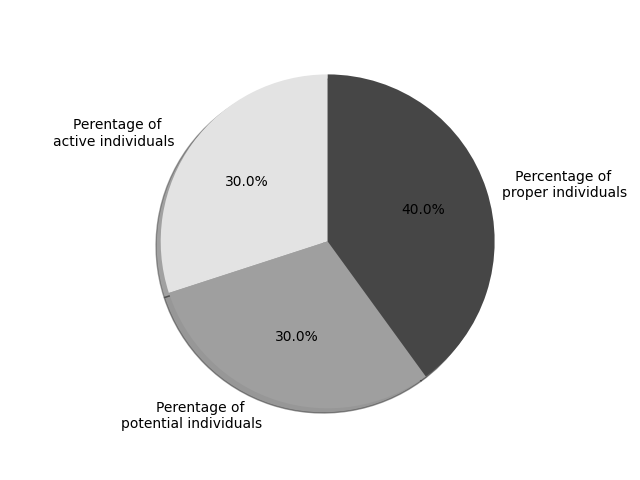
\includegraphics[width=\linewidth]{fig/percentage_of_groups}
	\caption{Percentage of active individuals from active group, potential
	  individuals from potential group, and proper individuals from proper group
	 in parent population.}
	\label{fig:group}
\end{figure}

\begin{table}[!htb]
\centering
\caption{Parameters of proposed GA model.}
\begin{adjustbox}{width=0.45\textwidth}
\label{tab:ga}
\begin{tabular}{lc}
\toprule
Parameter								&  Value  \\
\midrule
Population                              & 40        \\
Initial length range					& [3-15]    \\
Encoding								& Integer   \\
Percentage of parent                    & 0.5   \\
Percentage of active group				& 0.3   \\
Percentage of potential group			& 0.3   \\
Percentage of proper group				& 0.4   \\
Selection strategy for  active group	& Ranking   \\
Selection strategy for potential group	& Ranking   \\
Selection strategy for proper group	    & Ranking   \\
Crossover strategy			    		& One-point \\
Mutation strategy			    		& Mass mutation \\
Length mutation coefficient             & 5 \\
Angle mutation rate                     & 0.1 \\
\bottomrule
\end{tabular}
\end{adjustbox}
\end{table}



\subsection{Numerical Results and Discussion}
To figure out how the number of individuals in each group varies during the GA
process, we conduct one-time experiment and show the number of individuals
in each generation in respect of GA generation. Second, to verify its
performance and stability, the GA is run one hundred times: the best, worst
case, and average results are presented, respectively. Finally, we compare
the results with the work in the other literature.

\begin{figure}[!tb]
	\centering
	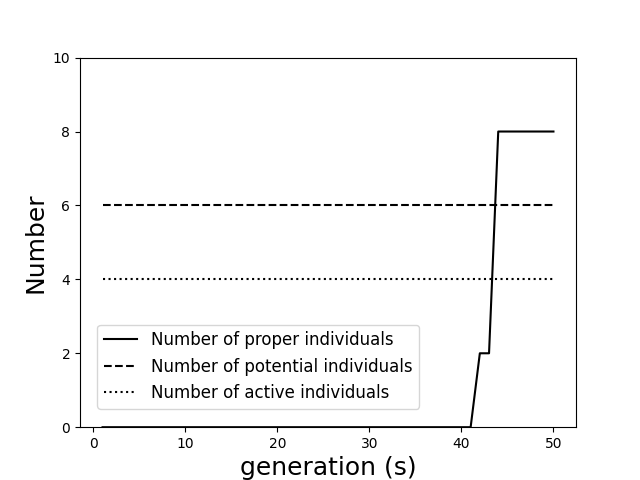
\includegraphics[width=\linewidth]{Figures/chapter4/part1/fig/group_number.png}
	\caption{Number of individuals in each group as a function of generation.}
	\label{fig:group}
\end{figure}

\begin{figure}[!tb]
	\centering
	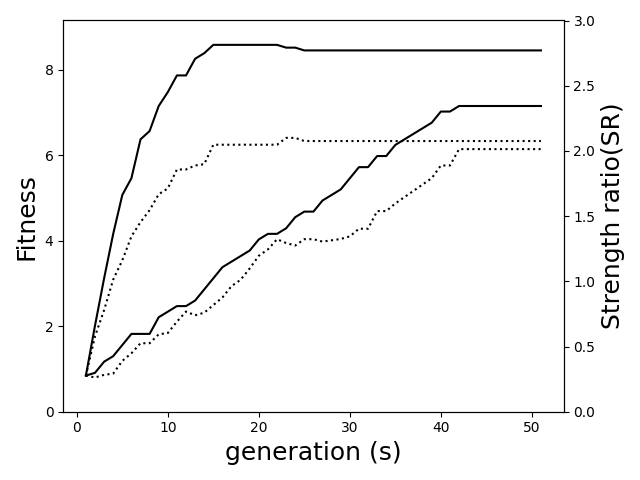
\includegraphics[width=\linewidth]{Figures/chapter4/part1/fig/fitness_strength_ratio.png}
	\caption{The fitness is the negation of the individual's mass. The solid
		curve is the fitness of the best individual in the population in respect
		to the generations; and the dotted line denotes its corresponding strength
		ratio. If no individuals in the population satisfy the constraint, the
		best individual is the one with the biggest strength ratio; if not, the
		best individual is the one with the smallest mass.
}
	\label{fig:sr}
\end{figure}



Fig. \ref{fig:group} shows the number of individuals in each group during the
one-time GA process.  For both active group and potential groups, the number of
individuals is fixed, and equal to its upper bound from the beginning to the
end of the searching process. However, for the proper group, at the initial
stage of GA, no individual fulfills the constraint, so the number of proper
individuals is zero. As seen from Fig. \ref{fig:group}, after forty
generations, proper individuals appear, and its population increases very
quickly up to its upper bound.

There are two approaches that the GA could obtain a better solution: the first
is increasing the length of the chromosome; the second one is adjusting the
internal structure of a chromosome. The GA process can be divided into two
phases by whether there are proper individuals or not. Fig.
\ref{fig:sr} shows the GA process in which the dashed vertical line is the
watershed between the initial phase and the last phase. In the initial phase,
no individual's strength ratio is over the specified threshold, and the main
reason that the fitness gets smaller gradually is the increase of chromosome's
length; At point 1 on the fitness curve, the fitness suddenly goes up, however,
the corresponding strength ratio of point 1, denoted by the point $1^{\prime}$
on the generation-strength ratio curve, also increases. it is because of the
adjustment of a chromosome's layup.  Then GA comes to its second phase. During
this phase, the GA already found proper individuals which could satisfy the
constraint, so the target in this stage is to improve fitness. This means GA
needs to adjust its inner structure, at the point 2 and 3 on the
generation-fitness curve, the fitness curves go up, and the corresponding
strength ratio of these two points slightly go down, but both of them still
satisfy the constraint.


\begin{table*}
\caption{The optimum lay-ups for the loading $N_x=1e^6$ N when changing the value length mutation coefficient, the performance of the GA can be improved when the lenght mutation coefficient is reduced to 1.}
\centering
\begin{adjustbox}{width=1\textwidth}
	\begin{tabular}{cccccccc}
	\toprule
	coefficient		     &	 Material		               	 & case     & Stacking sequence    & Strength ratio  & Mass  &  Cost   & Layer    \\ 
	\midrule																															  
	\multirow{6}{*}{1} &	\multirow{3}{*}{glass-epoxy}   	 & worst     &  $[0_{80}/90_{52}]$ & 2.010           &  8.58  & 132     & 132   \\
						 &								     & best      &  $[0_{75}/90_{43}]$ & 2.000           &  7.67  & 118     & 118  \\
					     &									 & average   &    		           & 2.012           &  7.83  & 123     & 123  \\
						 &	\multirow{3}{*}{graphite-epoxy}	 & worst     &  $[0_{17}/90_{15}]$ & 2.036           & 1.68   & 80      & 32      \\
					     &								     & best      &  $[0_{17}/90_{5}]$  & 2.005           & 1.15   & 55      & 22      \\
					     &								     & average   &                     & 2.018           & 1.47   & 70      & 28      \\
	\multirow{6}{*}{5} &	\multirow{3}{*}{glass-epoxy}   	 & worst     &  $[0_{72}/90_{64}]$ &  2.009          & 8.84   &  136    &  136   \\
						 &								     & best      &  $[0_{72}/90_{53}]$ &  2.003          & 8.12   &  125    &  125   \\
					     &									 & average   &                     &  2.008          & 8.55   &  131    &  131  \\
						 &	\multirow{3}{*}{graphite-epoxy}	 & worst     &  $[0_{18}/90_{24}]$ &  2.006          & 2.20   &  105    &  42  \\
					     &								     & best      &  $[0_{17}/90_{6}]$  &  2.001          & 1.20   &  57     &  23  \\
					     &								     & average   &                    &   2.022          & 1.54   &  73     &  29  \\
	\bottomrule																															  
\end{tabular}
\end{adjustbox}
\label{tab:optimum_layup}
\end{table*}
            
            

Tab. \ref{tab:optimum_layup} shows the searching results after conducting this
experiment one hundred times in two length mutation coefficient cases for
glass-epoxy and graphite-epoxy material, respectively. The best, worst case, and
average experiment results are showed in this table.  For the glass-epoxy
material, if the length mutation coefficient takes one, the best and worst
sequences are $[0_{40}/90_{26}]_s$, $[90_{24}/0_{38}/\bar{90}]_s$; the average mass, cost,
and number of layers are 7.83, 123, 123. If we increase its length mutation
coefficient, suppose it is five, the number of layers for best and worst cases
are 125 and 136;  the average mass, cost, and number of layers are 8.55, 131,
131.  When graphite-epoxy is taken as the experiment material, similar
experiment results are found.  Comparing these two results, we see that a
bigger value of length mutation coefficient can improve this GA's performance.
This is because the mutation coefficient can control both the convergence speed
and search performance, a small mutation coefficient would slow the convergence
speed, however, it would lead to a small-grained exploitation in the local space. 


\begin{table*}[!htb]
\caption{The optimum lay-ups for the loading $N_x=1e6$ N}
\centering
\begin{adjustbox}{width=1\textwidth}
\begin{tabular}{c|cc|cc}
	\toprule
	Cross Ply $[0_M/90_N]$         & \multicolumn{2}{c}{Previous Research} & \multicolumn{2}{c}{Current Research} \\
	\midrule																								  
	 Material       &  Glass-Epoxy & Graphite-Epoxy  & Glass-Epoxy & Graphite-Epoxy      \\ 
	      M         &  68          &    17           &  78		    &  18             \\
	      N         &  72          &    18           &  28		    &  8              \\
no. of lamina(n)    &  140         &    35           &  106	    &  26                     \\
         SR         &  2.01        &    2.10         &  2.03	    &  2.16            \\
     weight         &  9.10        &    1.84         &  6.89	    &  102.5           \\
	\bottomrule
\end{tabular}
\end{adjustbox}
\label{tab:comparsion}
\end{table*}

Tab. \ref{tab:comparsion} shows the optimal cross-ply sequences by the
proposed GA and  Choudhury and Mondal's\cite{choudhury2019failure} study. For
the loading case $Nx=1$ MPa m, the optimal layups are a $[0_{68}/90_{72}]$
cross-ply laminate if glass-epoxy is taken; however, in the present study, a
$[90_{24}/0_{38}/\bar{90}]_s$ glass-epoxy cross-ply laminate is found which
significantly reduces both the cost and weight, and it satisfies the
constraint.  Similarly, if graphite-epoxy is taken, compared with the
$[0_{17}/90_{18}]$ cross-ply laminate, an alternative solution is found,
its layup is $[0_{9}/90_{1}/\bar{0}]_s$. For both cases, we can see that the
experiment results show that using the present proposed GA can obtain better
results.

\section{conclusions}
In this paper, we reviewed the use of the proposed ga framework, classical
lamination theory, and tsai-wu failure theory for the lay-up design for
cross-ply laminate. Because GA is primarily used to solve an unconstrained
problem, and it is not suitable for a constrained problem. In the present
study, we deal with this constrained problem by mixing strategies of selection
methods instead of adding punishment terms into the objective function. So the
constraint problem can be solved in an unconstrained way.

This variant of the GA provides a new approach to address the constrained
search for optimization of laminated composite, and this method can be easy
to apply in other domains. At the same time, the proposed GA model is more
complicated than the traditional GA model, which involves more parameters. To
advance its performance, the fine-tuning of those parameters need more effort. 

\section*{Acknowledgment}
The paper was supported by China Scholarship Council with
the code number 201806630112



\bibliographystyle{SageV}
\bibliography{reference}

\end{document}
